\section{Algoritmos}
\label{sec:algoritmos}
\subsection{Introducción}
En esta sección vamos a explicar que algoritmos se han usado después del pre-procesamiento inicial.\\
Existe un teorema llamado\textbf{ \textit{No-Free-Lunch}} que afirma no existe un algoritmo que resuelva los problemas de machine learning mejor que otro.\\
Partiendo de esta idea, el objetivo principal de esta sección es el de comprobar el comportamiento de una serie de modelos elegidos. \\
De estos modelos, algunos se adaptaran mejor que otros para los datos con los que se trabajan. Una vez analizado el comportamiento, podremos decidir que algoritmos vamos a usar y que algoritmos van a ser descartados. \\
\linebreak
Para el caso especifico con el que se está trabajando, vemos que es un problema bastante peculiar, ya que esta formado por varias variables objetivo de tipo ordinal, añadiendo una nueva característica siendo esta la\textbf{media} de estas variables.\\
Para esta sección, se ha usado la media y se ha planteado un problema de \textbf{regresión}, en el que algoritmo, dada una entrada predecirá que valor medio de emprendimiento tiene esa persona.

\subsection{Métricas}
Para comprobar el comportamiento de nuestro modelo se usan \textbf{métricas}.  Las métricas que se han usado son \textit{\textbf{Coeficiente de determinación}} (se denota como $R^2$), \textit{\textbf{Desviación de Poisson}} y \textit{\textbf{Error cuadrático medio}}
\subsubsection{Coeficiente de determinación}
Se define como \textbf{coeficiente de determinación} como la proporción de la varianza total explicada por la variables independientes del modelo. Proporciona una indicación de como de bueno es un ajuste y por tanto, una medida de como de bueno es el modelo cuando predice nuevas muestras.\\
\linebreak
Matemáticamente, se define el coeficiente de determinación como:
\[
	R^2 (y, \hat{y}) = 1 - \frac{\sum_{i=1}^{n}(y_i - \hat{y}_i)^2}    {\sum_{i=1}^{n} (y_i - \overline{y})^2}
\]

Donde:
\begin{itemize}
	\item $y$ es el conjunto de valores reales para las variables objetivo.
	\item $\hat{y}$ es el valor predicho para los valores objetivo.
	\item $\hat{y}_i$ es la predicción de la  i-ésima muestra.
	\item $y_i$ es el valor real de la i-ésima muestra.
	\item $\overline{y} = \frac{1}{n} \sum_{i=1}^{n} y_i$.
	\item $n$ es el numero de muestras del conjunto.
\end{itemize}
insertar graficos explicando varianza,  etc
\subsubsection{Desviación de Poisson}
\subsubsection{Error cuadrático medio}
El error cuadrático medio de un estimador mide el promedio de los errores al cuadrado.  \\
Matemáticamente, se define el error cuadrático medio como:
\[
	MSE(y,\hat{y}) = \frac{1}{n} \sum_{i=1}^{n} (y_i - \hat{y}_i) ^2
\]
Donde:
\begin{itemize}
	\item $y$ es el conjunto de valores reales para las variables objetivo.
	\item $\hat{y}$ es el valor predicho para los valores objetivo.
	\item $\hat{y}_i$ es la predicción de la  i-ésima muestra.
	\item $y_i$ es el valor real de la i-ésima muestra.
	\item $n$ es el numero de muestras del conjunto.
\end{itemize}
\subsubsection{Conjuntos de validación}
Para ver el comportamiento de un modelo, se puede definir un conjunto de entrenamiento para entrenar el modelo que se ha seleccionado y un conjunto de test para comprobar el comportamiento con datos que el algoritmo no conoce.  Aunque a primera vista esta parece una técnica correcta, tiene varios inconvenientes:
\begin{itemize}
	\item Cuando se ajustan los hiper-parámetros de los modelos,  se podría llegar a ajustar el modelo al conjunto de test, produciendo un sobre-ajuste.
	\item Solo se esta usando una parte de los datos para validar el modelo, nada asegura que el conjunto de test sea representativo del conjunto de datos con el que se está trabajando.
\end{itemize}
Para solventar estas y algunos otros problemas que que tiene esta metodología, se usa la \textbf{validación cruzada}.\\
\linebreak
En vez de usar el conjunto de entrenamiento para entrenar un único modelo, se divide el conjunto de entrenamiento en $k$ partes, entrenando $k$ modelos usando $k-1$ subconjunto y usando el restante como de test. \\
 \begin{figure}[H]
	\centering
	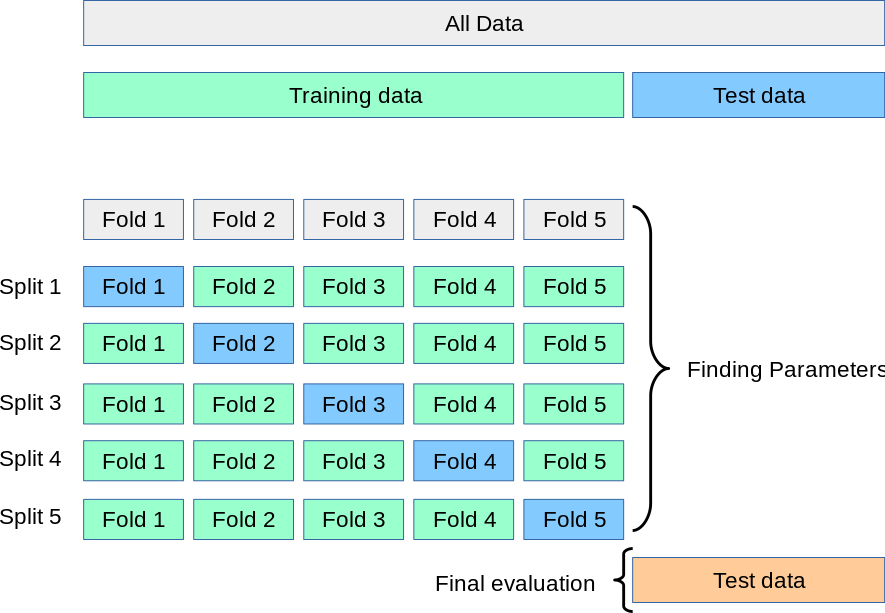
\includegraphics[scale=0.4]{grid_search_cross_validation.png}
	\caption{Ejemplo de validación cruzada con $k=5$}
	\label{fig:cross-validation}
\end{figure}
Como se aprecia en la figura \ref{fig:cross-validation},  se ha dividido el conjunto de datos en 5 conjuntos (folds), usando en cada iteración 4 para entrenar el modelo y uno para verificar con datos que el modelo no ha visto. Finalmente, se usa el conjunto de test (habiendo entrenado previamente el modelo con todo el conjunto de entrenamiento).
\subsubsection{Gráficos}
Además del uso de las métricas mencionadas previamente, se han creado las siguientes gráficas para visualizar los errores que esta haciendo un modelo en concreto. Esto ayuda a la toma de decisiones en fases siguientes.\\
Las gráficas que se han desarrollado son las siguientes:
\begin{itemize}
	\item Gráfico de dispersión de errores.
	\item Cantidad de errores por rango. (probablemente sea mejor cambiar este nombre, pero es el nombre que se me ocurrió)
\end{itemize}
El gráfico de dispersión de errores consiste en mostrar en la misma gráfica el valor real de las variables objetivo y el valor predicho por nuestro modelo. Esto nos permite ver como de juntos están las predicciones, identificando así en que zonas el algoritmo se está equivocando más frecuentemente.\\
 \begin{figure}[H]
	\centering
	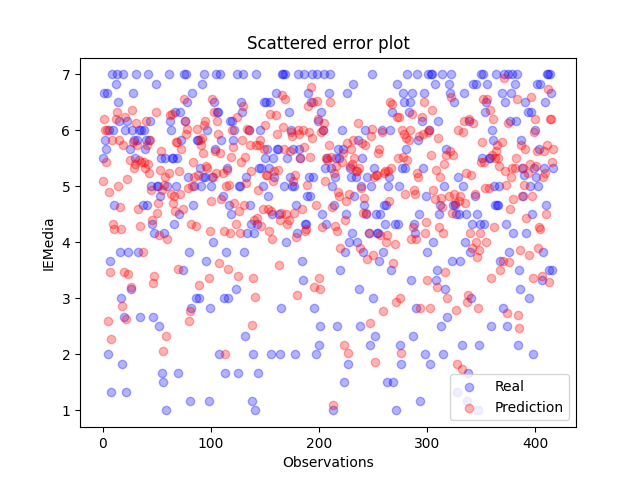
\includegraphics[scale=0.6]{scattered.png}
	\caption{Ejemplo de gráfico de dispersión de errores}
	\label{fig:scattered_example}
\end{figure}
El segundo gráfico consiste en lo siguiente:
Los modelos que han sido entrenados están prediciendo valores medios. El proceso o pseguidara realizar estos gráficos ha sido el de obtener el valor redondeado de la predicción y del valor real. Si la predicción y el dato real son distintos, se ha considerado como error y se han contado el número de errores para cada valor REAL redondeado.\\
Usando esta gráfica, se puede identificar fácilmente en que rangos los modelos están fallando.\\
\linebreak
 \begin{figure}[H]
	\centering
	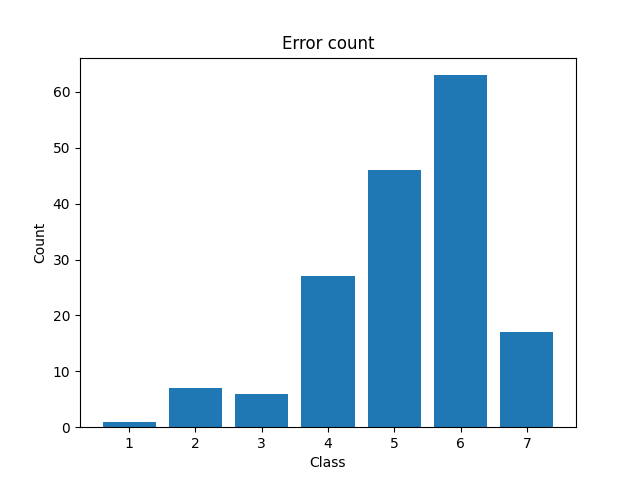
\includegraphics[scale=0.6]{error_hist.png}
	\caption{Ejemplo de gráfico de errores por rango}
	\label{fig:error_hist_example}
\end{figure}
\subsection{Árboles de decisión}
\label{alg:dec_tree}
Los árboles de decisión son modelos que predicen la variable objetivo usando reglas del tipo \textit{si variable cumple condición entonces } inferidas a partir de los datos con los que se entrena el algoritmo.\\
Los árboles de decisión ofrecen ciertas ventajas:
\begin{enumerate}
	\item Son modelos fáciles de interpretar y pueden ser visualizados.
	\item Son capaces de trabajar con variables categóricas y numéricas.
	\item introducir alguna ventaja más
\end{enumerate}
Sin embargo, estos modelos también presentan ciertas desventajas:
\begin{enumerate}
	\item Algoritmos que tienden al sobre-aprendizaje.
	\item No soportan valores perdidos.
	\item No trabajan bien con conjuntos de datos des-balanceados.
\end{enumerate}
Se ha seleccionado este algoritmo ya que es un algoritmo que a parte de predecir nuevos valores, puede proporcionar información extra sobre conjunto de datos (importancia de variables, variables que definen cierto grupo, etc).
\subsubsection{Procesado de datos}
Antes de ejecutar la fase de entrenamiento, hay que modificar los datos para adaptarlos a las limitaciones que algoritmo impone. En este caso,  los árboles de decisión no admiten valores perdidos y debido a ciertas limitaciones de la librería que se está usando, los árboles de decisión no son capaces de trabajar con variables categóricas.\\
Las modificaciones que se han hecho previamente son: (por orden)
\begin{enumerate}
	\item \textbf{Imputación de valores perdidos}
	\item \textbf{Transformación de variables categóricas a numéricas}
\end{enumerate}
 Por este motivo, se ha tenido que introducir una fase extra transformando las variables categóricas en numéricas.
\subsubsection{Resultados}
\label{sec:res_tree}
Antes de mostrar los resultados, hay que destacar que cuando se entrena un árbol de decisión sin limitar los parámetros, este va a seguir separando los datos de entrenamiento hasta que no pueda realizar más divisiones. Para encontrar el árbol óptimo, primero se ha entrenado el árbol por defecto y se han obtenido los parámetros. Esos parámetros se han establecido como limite, se han entrenado varios árboles con distintos parámetros (sin superar el límite establecido por el primer modelo) y se ha escogido el que mejores resultados obtenía. Los parámetros que mejor resultados dieron son: \\
\begin{itemize}
	\item \textbf{Profundidad máxima:} Limita la profundidad (cantidad de preguntas) del árbol. El mejor valor ha sido \textbf{8}
	\item \textbf{Máximo número de hojas:} Máximo numero de hojas (grupos en el último nivel de una rama). El mejor valor ha sido \textbf{16}
\end{itemize}
En esta sección se va a exponer los resultados obtenidos usando el algoritmo de \textbf{árboles de decisión}.\\
La siguiente tabla expone los resultados obtenidos en validación:
\begin{table}[htbp]
    \begin{tabular}{|c|c|c|c|c}
    \cline{1-4}
    Métricas         & R2    & Poisson deviance & MSE   \\ \cline{1-4}
    FOLD 1           & 0.678 & 0.211            & 0.886 \\ \cline{1-4}
    FOLD 2           & 0.65  & 0.213            & 0.913 \\ \cline{1-4}
    FOLD 3           & 0.629 & 0.239            & 0.98  \\ \cline{1-4}
    FOLD 4           & 0.679 & 0.187            & 0.779 \\ \cline{1-4}
    FOLD 5           & 0.636 & 0.211            & 0.933 \\ \cline{1-4}
    Media Validación & 0.654 & 0.212            & 0.898 \\ \cline{1-4}
    Test             & 0.69  & 0.196            & 0.815 \\ \cline{1-4}
    \end{tabular}
	\caption{Árbol de decisión:  Profundidad 8, número máximo de hojas 16}
	\label{tab:tree_res}
\end{table}
La siguiente figura muestra el gráfico de dispersión de errores:\\
 \begin{figure}[H]
	\centering
	\includegraphics[scale=0.8]{src/scattered_error_dtree.png}
	\caption{Gráfico de dispersión de errores}
	\label{fig:tree_scattered}
\end{figure}
Continuando con las gráficas, e continuación se muestra una gráfica con el conteo de errores por clase:
 \begin{figure}[H]
	\centering
	\includegraphics[scale=0.8]{src/error_hist_dtree.png}
	\caption{Conteo de errores}
	\label{fig:tree_error_plot}
\end{figure}
\subsubsection{Representación}
Como se mencionó en la sección \textbf{\ref{alg:dec_tree}-\nameref{alg:dec_tree}}, los árboles de decisión tienen la ventaja de que pueden representarse fácilmente. \\
En este caso, vamos a usar una representación gráfica del árbol, las reglas que ha obtenido el árbol y las variables más importantes.\\
\linebreak
La siguiente figura muestra la representación gráfica del árbol de decisión entrenado:\\
\linebreak
 \begin{figure}[H]
	\centering
	\includegraphics[scale=0.2]{src/decision_tree_plot.png}
	\caption{Árbol de decisión}
	\label{fig:decission_tree1}
\end{figure}
A continuación se muestra en pseudo-código, las reglas que ha inferido el árbol de decisión:\\

\begin{figure}[H]
	\begin{lstlisting}
def predict(sample):
	if AE5 <= 4.5:
		if AcMedia <= 3.1:
			if AE5 <= 1.5:
				return 1.28
			else:  # if AE5 > 1.5
				return 2.12
		else:  # if AcMedia > 3.1
			if SE2 <= 3.5:
				if BA3.f <= 0.5:
					return 3.27
				else:  # if BA3.f > 0.5
					return 4.61
			else:  # if SE2 > 3.5
				if Beca <= 0.75:
					if Nota <= 6.85:
						return 3.46
					else:  # if Nota > 6.85
						return 4.52
				else:  # if Beca > 0.75
					return 3.32
	else:  # if AE5 > 4.5
		if AE5 <= 5.75:
			if SE2 <= 3.5:
				if CEF19 <= 3.75:
					return 4.7
				else:  # if CEF19 > 3.75
					return 3.79
			else:  # if SE2 > 3.5
				return 5.19
		else:  # if AE5 > 5.75
			if AcMedia <= 6.55:
				if SE5 <= 1.5:
					return 2.75
				else:  # if SE5 > 1.5
					if NS1 <= 6.75:
						return 5.5
					else:  # if NS1 > 6.75
						if AE7 <= 2.75:
							return 4.69
						else:  # if AE7 > 2.75
							return 6.13
			else:  # if AcMedia > 6.55
				if SEMedia <= 3.58:
					return 5.68
				else:  # if SEMedia > 3.58
					return 6.6
	\end{lstlisting}
\caption{Reglas del árbol de decisión}
\label{fig:tree_rules}
\end{figure}
\pagebreak
Por ultimo, estas son las 10 variables que el modelo consideró con más relevancia. El valor asociado a cada variable es la \textbf{importancia Gini}:
\begin{figure}[H]
	\centering
	\includegraphics[scale=0.25]{src/feature_importance_dtree}
	\caption{10 variables más importantes segun AD}
	\label{fig:feature_dtree}
\end{figure}
Volviendo a la documentación proporcionada para comprobar el significado de esos valores:
\begin{itemize}
	\item \textbf{AE5:} Pregunta  5 sobre Actitudes financieras empresariales. Valor $0.735667$
	\item \textbf{AcMedia:} Variable global de Actitud emprendedora. Valor $0.156046$
	\item \textbf{SE2:} Estoy preparado para iniciar una empresa viable. Valor $0.037300$
	\item \textbf{SE5:} Conozco cómo desarrollar un proyecto empresarial. Valor $0.014692$
	\item \textbf{NS1:} Mi familia aprobaría el que yo decidiese crear una empresa. Valor $0.012393$
	\item \textbf{Beca:} Tiene beca el encuestado. Valor $0.008256$
	\item \textbf{Nota:} Nota media del expediente académico hasta la fecha de la encuesta sobre 10 puntos. Valor $0.008034$
	\item \textbf{BA3.f:} En los últimos 12 meses, ¿has ahorrado personalmente algún dinero de alguna de las siguientes formas, independientemente de si aún dispones del dinero? Han contestado las opciones a, c, d, e, f, g (en casa, en cuenta de ahorro, darlo a la familia, productos de inversión, de otro modo). Valor $0.007389$
	\item \textbf{CEF19:} Pregunta sobre Conocimientos financieros empresariales. Valor $0.007202$
	\item \textbf{AE7:} Pregunta 7 sobre Actitudes financieras empresariales. Valor $0.006518$
\end{itemize}
De las columnas \textit{AEx} y \textit{CEFx} no hay información en la documentación, unicamente se menciona que son una serie de preguntas relacionadas con actitudes financieras empresariales y sobre conocimientos financieros empresariales respectivamente.
\subsection{Random Forest}
Random Forest es un modelo  combinado de aprendizaje que puede usarse para clasificación y/o regresión. Random Forest consiste en un conjunto de árboles de decisión que operan juntos. Una vez que cada árbol dentro del Random Forest realiza una predicción, se escoge la predicción con más votos. \\ Se ha escogido este modelo ya que como se comprobó en la sección \textbf{\ref{alg:dec_tree}-\nameref{alg:dec_tree}}, los árboles de decisión dieron buenos resultados
\linebreak
Para que Random Forest funciona bien, hay que asegurar que los distintos árboles que lo forman tengan una baja \textbf{correlación} entre ellos. Esto quiere decir que los árboles tienen que diferir y proporcionar predicciones distintas, de esta manera, si hay un conjunto de  árboles que da una predicción malas, puede haber otro conjunto que vaya en la dirección correcta. \\
\linebreak
Los árboles de decisión son algoritmos que son muy sensibles a los datos con los que se ha entrenado, por lo que cualquier cambio en los datos de entrenamiento puede hacer que cambie una predicción. Random Forest hace uso de esta peculiaridad de los árboles de decisión.
En el momento de entrenar los distintos árboles, en vez de usar subconjuntos del conjunto de entrenamiento se usan $N$ conjuntos del mismo tamaño que el conjunto de entrenamiento obtenidos usando un \textbf{muestreo con reemplazo}. Una vez que se tienen los distintos conjuntos, se entrena cada conjunto con un árbol. Este proceso se conoce como \textbf{bagging}.\\
\linebreak
Una peculiaridad más que tiene Random Forest es la forma con la que los árboles seleccionan la variable que van a usar para dividir el conjunto de datos. Estos no eligen la variable en función de un criterio concreto, si no que eligen la variable usando un conjunto aleatorio de las características.  Esto fuerza a que los árboles sean mas diferentes entre ellos, bajando la correlación entre los árboles que forman el modelo.
\subsubsection{Procesado de datos}
Al igual que los árboles de decisión, se ha hecho una imputación de valores perdidos y se ha transformado las variables categóricas a numéricas debido a limitación que hay en la librería usada.
\pagebreak
\subsubsection{Resultados}
Antes de mostrar los resultados, estos son los parámetros que se han usado al entrenar el algoritmo:
\begin{itemize}
	\item \textbf{max\_features}:  Número de variables que se van a escoger de manera aleatoria: $\frac{1}{3}$ del número de variables.
	\item\textbf{n\_estimators}: Número de árboles que forman el Random Forest: $500$
\end{itemize}
En la siguiente tabla, se muestra el resultado para obtenidos en validación y en test:
\linebreak
\begin{table}[H]
	\centering
	\begin{tabular}{|c|c|c|c|c}
		\cline{1-4}
		Métricas          & R2    & Poisson deviance & MSE   \\ \cline{1-4}
		FOLD 1            & 0.765 & 0.156            & 0.647 \\ \cline{1-4}
		FOLD 2            & 0.778 & 0.136            & 0.577 \\ \cline{1-4}
		FOLD 3            & 0.735 & 0.174            & 0.7   \\ \cline{1-4}
		FOLD 4            & 0.732 & 0.152            & 0.65  \\ \cline{1-4}
		FOLD 5            & 0.751 & 0.147            & 0.639 \\ \cline{1-4}
		Media  Validación & 0.752 & 0.153            & 0.643 \\ \cline{1-4}
		Test     		  & 0.768  & 0.15            & 0.609 \\ \cline{1-4}
	\end{tabular}
	\caption{Random Forest}
	\label{tab:res_random_forest}
\end{table}
La siguiente figura muestra el gráfico de dispersión de errores:\\
\linebreak
\begin{figure}[H]
	\centering
	\includegraphics[scale=0.7]{src/scattered_error_random_forest.png}
	\caption{Gráfico de dispersión de errores}
	\label{fig:rf_scattered}
\end{figure}
Continuando con las gráficas, e continuación se muestra una gráfica con el conteo de errores por clase:
\begin{figure}[H]
	\centering
	\includegraphics[scale=0.7]{src/error_hist_random_forest.png}
	\caption{Conteo de errores}
	\label{fig:rf_error_plot}
\end{figure}
Para finalizar, esta es la lista de las 10 variables más importantes que ha obtenido Random Forest:
\begin{figure}[H]
	\centering
	\includegraphics[scale=0.6]{src/feature_importance_rf}
	\caption{10 variables más importantes según RF}
	\label{fig:feature_rf}
\end{figure}
Volviendo a la documentación, esta es la explicación para cada variable:
\begin{itemize}
	\item\textbf{AE5:} Pregunta  5 sobre Actitudes financieras empresariales. Valor = $0.246364$
	\item\textbf{AcMedia:} Variable global de Actitud emprendedora. Valor = $0.220202$
	\item\textbf{AC2:} Ser emprendedor es una salida profesional atractiva para mí. Valor = $0.072907$
	\item\textbf{AC4:}Ser emprendedor supondría una gran satisfacción para mí. Valor = $0.065776$
	\item\textbf{AC3:} Si tuviera la oportunidad y los recursos, me gustaría iniciar una empresa. Valor = $0.041642$
	\item\textbf{SEMedia:} Variable global de Autoeficacia emprendedora. Valor = $0.022872$
	\item\textbf{SE2:} Estoy preparado para iniciar una empresa viable. Valor = $0.019630$
	\item\textbf{AC1:} Ser emprendedor implica más ventajas que desventajas para mí. Valor = $0.019396$
	\item\textbf{NS1:} Mi familia aprobaría el que yo decidiese crear una empresa. Valor = $0.014467$
	\item\textbf{Nota:} Nota media del expediente académico hasta la fecha de la encuesta sobre 10 puntos. Valor = $0.012254$
\end{itemize}
\subsection{KNN}
\label{alg:knn}
El algoritmo  KNN (\textit{K Nearest Neighbors}) es un algoritmo supervisado basado en instancias. Este algoritmo no aprende un modelo si no que almacena todas las muestras de entrenamiento y cuando hay que predecir una nueva ejemplo, el algoritmo usa las muestras almacenadas calculando la distancia a cada muestra y obteniendo los K vecinos más cercanos y usando las etiquetas de los vecinos, asigna una predicción al ejemplo a predecir, generalmente asignando aquella clase con más "votos".\\
\linebreak
Para medir la distancia entre dos muestras, KNN puede usar una gran cantidad métricas, las más comunes son:
\begin{itemize}
	\item \textbf{Distancia euclidiana:} Definida como $\sqrt{\sum(x_1 - x_2)^2}$
	\item \textbf{Distancia Manhattan:} Definida como $\sum|x_1 - x_2|$
	\item \textbf{Distancia Minkowski:} Definida como $(\sum|x_1 - x_2|^p)^{\frac{1}{p}}$, siendo P un entero positivo
\end{itemize}
La implementación del algoritmo KNN de ScikitLearn usa por defecto la distancia \textbf{Minkowski}. Esta tiene la peculiaridad de que cambiando el parámetro $p$ puede usarse la distancia euclidiana ($p=2$) o la distancia Manhattan ($p=1$)
\subsubsection{Procesado de datos}
KNN es un algoritmo que depende de la distancia entre dos muestras, esto implica que si una caracteristica del conjunto de datos que se esta usando tiene un rango \textbf{mayor} que otra, esa característica aportará más al cálculo de la distancia, cuando no necesariamente debe de ser así. Por ese motivo, este algoritmo necesita que el conjunto de datos esté \textbf{normalizado} en el momento de entrenar.\\
\linebreak
Este algoritmo, a parte de necesitar que los datos estén normalizados, no admite valores perdidos y variables categóricas.
\subsubsection{Resultados}
Antes de mostrar los resultados, estos son los parámetros que se han usado al entrenar el algoritmo:
\begin{itemize}
	\item \textbf{K:} Número de vecinos: 5
	\item \textbf{Métrica:} Distancia usada: Minkowski con $P=2$ (distancia euclidiana).
\end{itemize}
En la siguiente tabla, se muestra el resultado para obtenidos en validación y en test:
\linebreak
\begin{table}[H]
	 \centering
	\begin{tabular}{|c|c|c|c|c}
		\cline{1-4}
		Métricas         & R2    & Poisson deviance & MSE   \\ \cline{1-4}
		FOLD 1           & 0.47  & 0.356            & 1.46  \\ \cline{1-4}
		FOLD 2           & 0.407 & 0.378            & 1.545 \\ \cline{1-4}
		FOLD 3           & 0.449 & 0.362            & 1.457 \\ \cline{1-4}
		FOLD 4           & 0.435 & 0.329            & 1.372 \\ \cline{1-4}
		FOLD 5           & 0.467 & 0.321            & 1.367 \\ \cline{1-4}
		Media Validación & 0.446 & 0.349            & 1.44  \\ \cline{1-4}
		Test             & 0.527 & 0.301            & 1.242 \\ \cline{1-4}
	\end{tabular}
	\caption{KNN: $K=5$, métrica Minkowski con $P=2$}
	\label{tab:knn_res}
\end{table}
La siguiente figura muestra el gráfico de dispersión de errores:
\begin{figure}[H]
	\centering
	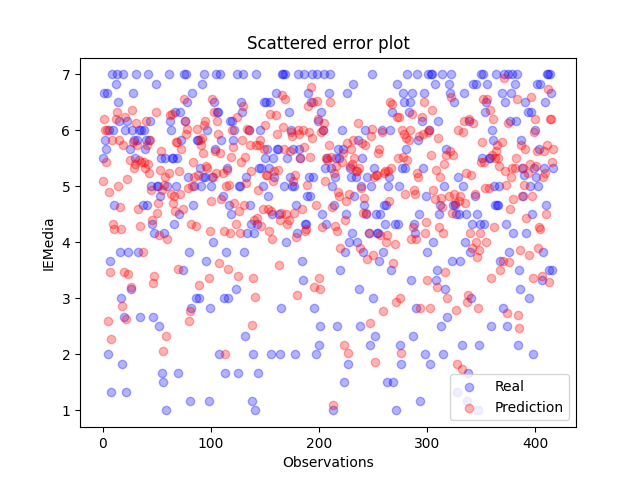
\includegraphics[scale=0.8]{src/scattered_error_knn.png}
	\caption{Gráfico de dispersión de errores}
	\label{fig:knn_scattered}
\end{figure}
Continuando con las gráficas, e continuación se muestra una gráfica con el conteo de errores por clase:\\
\linebreak
\begin{figure}[H]
	\centering
	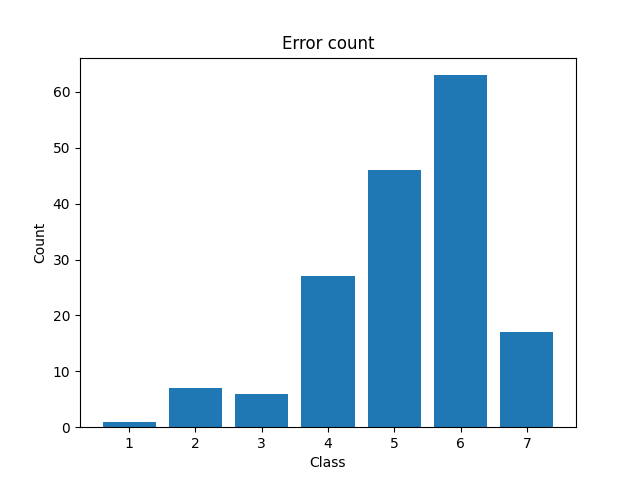
\includegraphics[scale=0.8]{src/error_hist_knn.png}
	\caption{Conteo de errores}
	\label{fig:knn_error_plot}
\end{figure}
\subsection{SVM}
\subsubsection{Procesado de datos}
\subsubsection{Resultados}
\begin{table}[H]
	  \centering
	\begin{tabular}{|l|l|l|l|l}
		\cline{1-4}
		Métricas         & R2      & Poisson deviance & MSE   \\ \cline{1-4}
		FOLD 1   		 & 0.671   & 0.236            & 0.906 \\ \cline {1-4}
		FOLD 2   		 & 0.718   & 0.186            & 0.734 \\ \cline {1-4}
		FOLD 3   		 & 0.728   & 0.185            & 0.72  \\ \cline {1-4}
		FOLD 4   		 & 0.691   & 0.192            & 0.75  \\ \cline {1-4}
		FOLD 5   		 & 0.697   & 0.193            & 0.776 \\ \cline {1-4}
		Media Validación & 0.701   & 0.198            & 0.777 \\ \cline {1-4}
		Test             & 0.737   & 0.173            & 0.691 \\ \cline {1-4}
	\end{tabular}
\caption{SVM: Tolerancia $1^{-3}$, Kernel RBF, $C=1$}
\label{tab:svm_res}
\end{table}
La siguiente figura muestra el gráfico de dispersión de errores:
\begin{figure}[H]
	\centering
	\includegraphics[scale=0.8]{src/scattered_error_svr.png}
	\caption{Gráfico de dispersión de errores}
	\label{fig:svr_scattered}
\end{figure}
Continuando con las gráficas, e continuación se muestra una gráfica con el conteo de errores por clase:\\
\linebreak
\begin{figure}[H]
	\centering
	\includegraphics[scale=0.8]{src/error_hist_svr.png}
	\caption{Conteo de errores}
	\label{fig:svr_error_plot}
\end{figure}
\subsection{XGBoost}
\subsubsection{Procesado de datos}
\subsubsection{Resultados}
\begin{table}[H]
	 \centering
	\begin{tabular}{|l|l|l|l|l}
		\cline{1-4}
		Métricas         &	 R2  & Poisson deviance & MSE   \\ \cline{1-4}
		FOLD 1           & 0.724 & 0.188            & 0.759 \\ \cline{1-4}
		FOLD 2           & 0.73  & 0.166            & 0.704 \\ \cline{1-4}
		FOLD 3           & 0.712 & 0.195            & 0.761 \\ \cline{1-4}
		FOLD 4           & 0.72  & 0.162            & 0.679 \\ \cline{1-4}
		FOLD 5           & 0.744 & 0.156            & 0.658 \\ \cline{1-4}
		Media Validación & 0.726 & 0.173            & 0.712 \\ \cline{1-4}
		Test             & 0.74  & 0.163            & 0.682 \\ \cline{1-4}
	\end{tabular}
\end{table}
La siguiente figura muestra el gráfico de dispersión de errores:
\begin{figure}[H]
	\centering
	\includegraphics[scale=0.8]{src/scattered_error_xgboost.png}
	\caption{Gráfico de dispersión de errores}
	\label{fig:xgboost_scattered}
\end{figure}
Continuando con las gráficas, e continuación se muestra una gráfica con el conteo de errores por clase:\\
\linebreak
\begin{figure}[H]
	\centering
	\includegraphics[scale=0.8]{src/error_hist_xgboost.png}
	\caption{Conteo de errores}
	\label{fig:xgboost_error_plot}
\end{figure}
\subsection{Perceptrón multicapa}
\subsubsection{Procesado de datos}
\subsubsection{Resultados}
\begin{table}[htbp]
	\begin{tabular}{|l|l|l|l|l}
		\cline{1-4}
		Métricas         & R2    & Poisson deviance & MSE   \\ \cline{1-4}
		FOLD 1           & 0.569 & 0.275            & 1.187 \\ \cline{1-4}
		FOLD 2           & 0.652 & 0.23             & 0.907 \\ \cline{1-4}
		FOLD 3           & 0.609 & 0.255            & 1.033 \\ \cline{1-4}
		FOLD 4           & 0.401 & 0.279            & 1.454 \\ \cline{1-4}
		FOLD 5           & 0.567 & 0.251            & 1.112 \\ \cline{1-4}
		Media Validación & 0.56  & 0.258            & 1.139 \\ \cline{1-4}
		Test	         & 0.625 & 0.244            & 0.984 \\ \cline{1-4}
	\end{tabular}
	\caption{Perceptrón Multicapa: 2 capas de 100 neuronas, 500 iteraciones}
	\label{tab:mlp_res}
\end{table}
La siguiente figura muestra el gráfico de dispersión de errores:
\begin{figure}[H]
	\centering
	\includegraphics[scale=0.8]{src/scattered_error_MLP.png}
	\caption{Gráfico de dispersión de errores}
	\label{fig:mlp_scattered}
\end{figure}
Continuando con las gráficas, e continuación se muestra una gráfica con el conteo de errores por clase:\\
\linebreak
\begin{figure}[H]
	\centering
	\includegraphics[scale=0.8]{src/error_hist_MLP.png}
	\caption{Conteo de errores}
	\label{fig:mlp_error_plot}
\end{figure}
\subsection{Conclusiones}
Se ha observado que los algoritmos basados en árboles de decisión se han comportado bien, por lo que se ha optado por seguir haciendo uso tanto de árboles de decisión como de Random Forest. Respecto a XGBoost, se ve que se tiene unos resultados ligeramente peores respecto a Random Forest pero con un comportamiento similar (tiene una cantidad considerable de fallos en valores altos de intención emprendedora media). Como XGBoost no esta aportando nada nuevo, por ahora se va a descartar.\\
\linebreak
SVR se ha comportado casi al nivel de algoritmos como XGBoost o Random Forest. Por ahora, no se va a descartar su uso, ya que introduciendo el conocimiento que se ha obtenido usando algoritmos como Random Forest o árboles de decisión se podría mejorar el rendimiento.\\
\linebreak
Respecto al algoritmo KNN,  se ve por los resultados que este algoritmo no funciona bien con nuestro conjunto de datos. La razón más probable por la que KNN obtuvo estos resultados, es que hay relaciones entre las variables que KNN no es capaz de detectar al únicamente comparar la distancia característica por característica. Debido al bajo desempeño que se ha obtenido al usar este algoritmo, este va a ser descartado de las siguientes fases.\\
\linebreak
Respecto al perceptrón multicapa, debido al rendimiento en comparación con otros algoritmos probados y debido al enorme coste de entrenamiento que pueden llegar a tener este algoritmo para que tenga un buen rendimiento, se ha decidido no continuar con este modelo\\
\linebreak
Como ya se ha mencionado, los modelos basados en árboles de decisión son capaces de obtener la importancia de las características. A continuación se muestran las gráficas de nuevo para facilitar la comparación:
\begin{figure}[H]
	\centering
	\includegraphics[scale=0.5]{src/feature_importance_dtree}
	\caption{10 variables más importantes según árboles de decisión}
	\label{fig:feature_dtree2}
\end{figure}
\begin{figure}[H]
	\centering
	\includegraphics[scale=0.5]{src/feature_importance_rf}
	\caption{10 variables más importantes según RF}
	\label{fig:feature_rf2}
\end{figure}
Como se ve en las figuras, vemos que hay dos variables que \textbf{ambos} algoritmos han dado como más importantes:
\begin{itemize}
	\item\textbf{AE5:} Pregunta  5 sobre Actitudes financieras empresariales.
	\item\textbf{AcMedia:} Variable global de Actitud emprendedora.
\end{itemize} 
Repasando los resultados obtenidos por los algoritmos, se ve claramente que a todos los algoritmos usados les está costando predecir correctamente los valores altos para la intención emprendedora media.
 \\
\linebreak
Por ejemplo, para el algoritmo que mejores resultados ha dado, ha tenido una alta cantidad de fallos para  valores altos (véase figura \ref{fig:rf_error_plot}). Este comportamiento ha sido constante para cada algoritmo usado. Una de las causas de este comportamiento puede ser explicada mediante las gráficas de dispersión de errores (véase figura \ref{fig:rf_scattered} para Random Forest). En esta figura se puede ver como, a medida que se incrementa el valor de intención emprendedora media, los datos son menos dispersos y a los algoritmos les está costando distinguir entre varios valores cercanos.
